\section{Hand detection}
Because of our settings, there are only white background, shadow and the hand in an image.
First, we detect hand using skin color. Then we detect wrist. Because there are only hand or wrist in the scene, we can get hand mask by erasing wrist region. Fig.\ref{fig:hand} shows the overview of the system. For wrist detection, we modify the method from \cite{ra11}.
All of the functions in this section is in major.py and hand\_detection.py.
\subsection{Skin color detection}
Because of our settings, there are only white background, shadow and the hand in an image.
So we detect the hand by color. We use both RGB and HSV value to detect our skin.
Because both of our team mates are East Asian, we tried skin detection only for East Asian people.
In particular, we define skin color pixel as:
\begin{itemize}
  \item its Red value is larger than Blue value
  \item its Red value is larger than Green value
  \item its Value (HSV) is smaller than 73 \%
  \item its Saturation is larger than 30 \%
 \end{itemize}
Also we mask where outside of the canvas.
\subsection{Orientaiton of the hand}
We want to detect the orientation of the hand in order to use training data, or detecting hand region.
In our program, majoraxis.py has this function.
We define the orientation of the hand as the angle of the axis of least second moment.\par
The input is the binary image of skin region.
Axis of least second moment minimizes E, the sum of the distance from all points to the line. That is,
$$E = \int \int r^2 b(x,y) dxdy$$
where $r$ is a distance from b(x,y) to the axis and b(x,y) = 1 when a pixel (x,y) belongs to the object, otherwise 0.
Let the axis be $x\sin{\theta} - y\sin{\theta} + \rho = 0$.
Distance of point (x,y) from axis is:
$$r = |x\sin{\theta}-y\cos{\theta}+\rho|$$.
Thus minimizing $E$ means minimizing
$$E = \int\int (x\sin{\theta}-y\cos{\theta}+\rho)^2 b(x,y)dxdy$$
Because $\partial E / \partial \rho = 0$, we get
$$A(x_c \sin{\theta} - y_c \cos{\theta} + \rho) = 0$$
where $A$ is an area of the object and $(x_c,y_c)$ is center of the object.
This means, the axis should pass the center point of the object.
Then, we shift the coordinate system in order to set the center point as origin.
That is, 
$x'= x - x_c, y' = y - y_c$.
Because this line should pass the origin, the line can be represented as
$x'\sin{\theta}-y'\cos{\theta}$
So, $$E = a \sin^2{\theta} - b\sin{\theta}\cos{\theta} + c\cos^2{\theta}$$.
Where $a = \int\int (x')^2 b(x,y) dx'dy', b = 2\int\int x'y' b(x,y) dx'dy', 
c = \int\int (y')^2 b(x,y)dx'dy'$.\par
Because $\partial E / \partial \theta = 0$, we get
$$(a-c)\sin{2\theta} - b\cos{2\theta} = 0$$
Also, minimizing E means the second derivative is larger than 0.
Using these information, the orientation $\theta = atan2(b,a-c)/2$.\par
Fig.\ref{fig:mom2} shows the results of orientation detection and the rotated image.
The first column is an original image.
The second column is a translated image. First, the center point of the hand moves to the center point of the image.
The light blue line is the axis. The blue dot is the center point.\par
When we return Then the image is rotated by the angle of $-\theta$.
This shows that this axis does not depends on the small fingertip movement.
If the binary image of hand has enough amount of areas, this system can detect the angle of the hand.
If the image of hand does not have enough amount of areas, for example, it can detect only a part of fingers,
it cannot detect the angle of the hand correctly.
However, because of our settings, we always can see enough amount of hand in the target area.
\begin{figure}
 \begin{tabular}{ll}
 Original image & Rotated hands \\
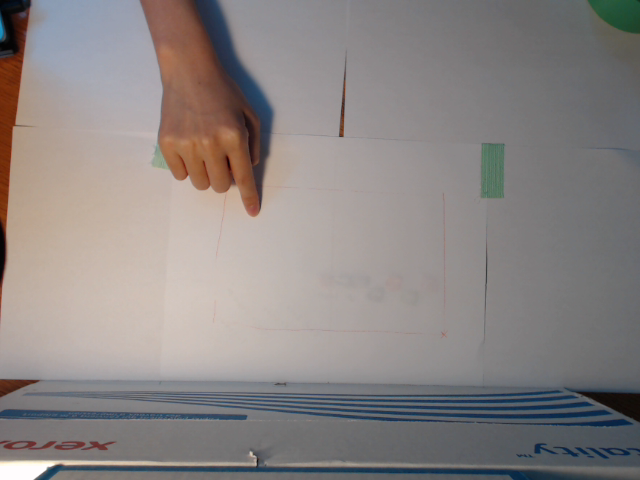
\includegraphics[width=5cm]{fig7/1-b.png} &
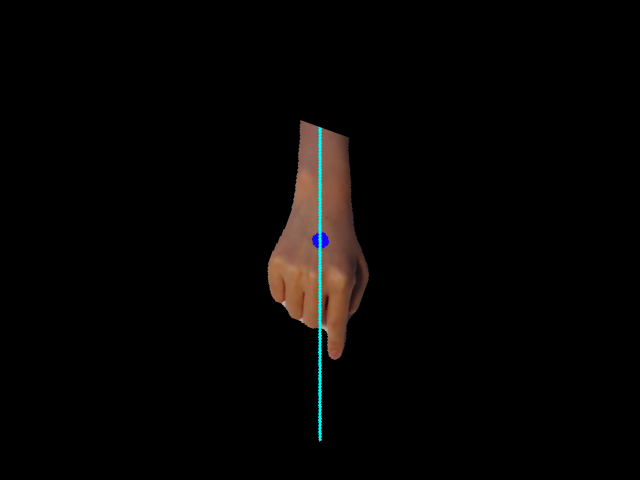
\includegraphics[width=5cm]{fig7/1-a.png} \\
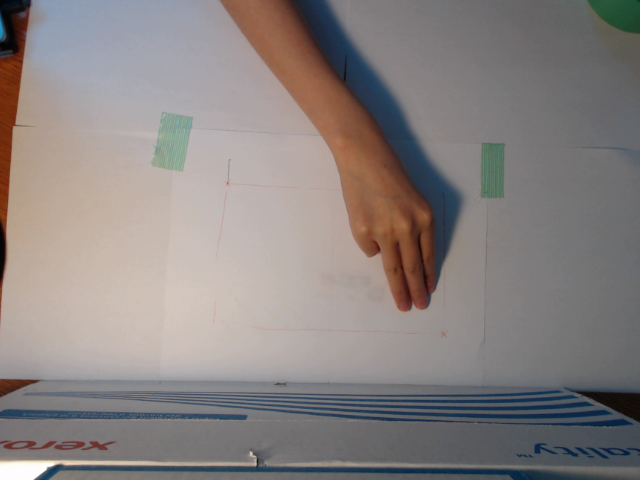
\includegraphics[width=5cm]{fig7/2-b.png} &
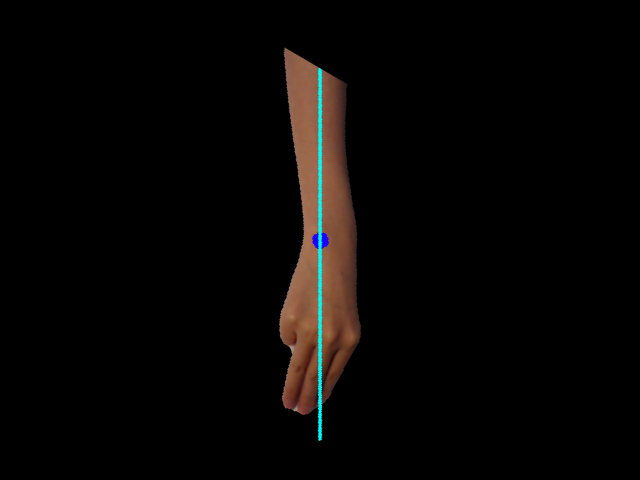
\includegraphics[width=5cm]{fig7/2-a.png} \\
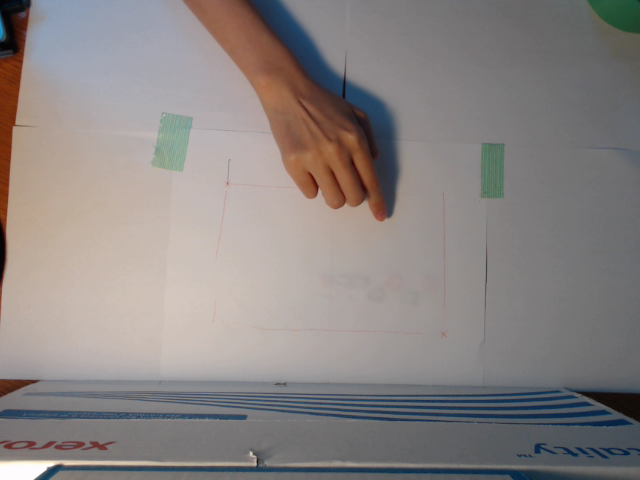
\includegraphics[width=5cm]{fig7/3-b.png} &
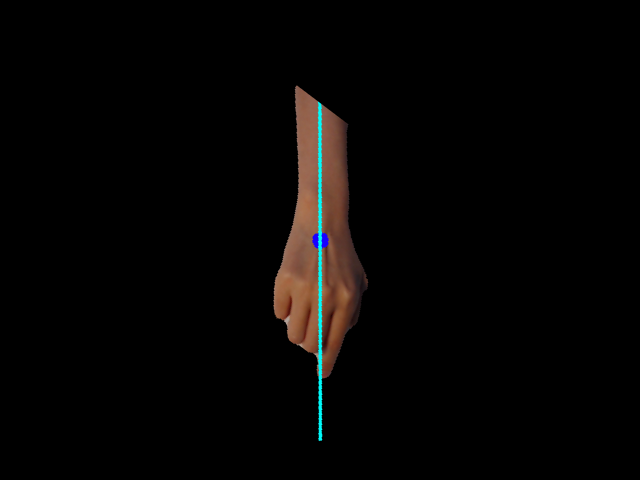
\includegraphics[width=5cm]{fig7/3-a.png} \\
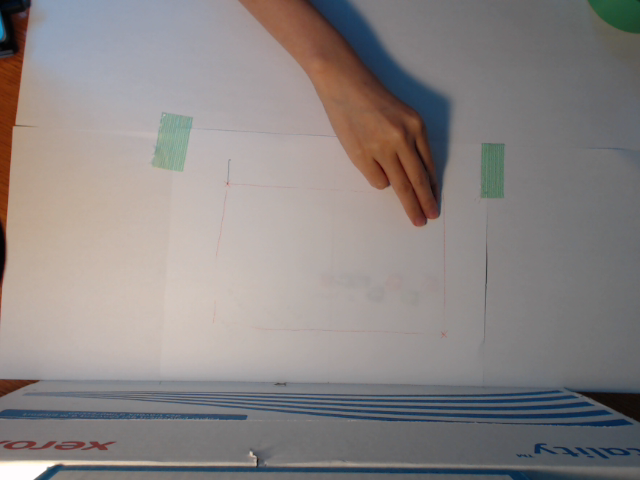
\includegraphics[width=5cm]{fig7/4-b.png} &
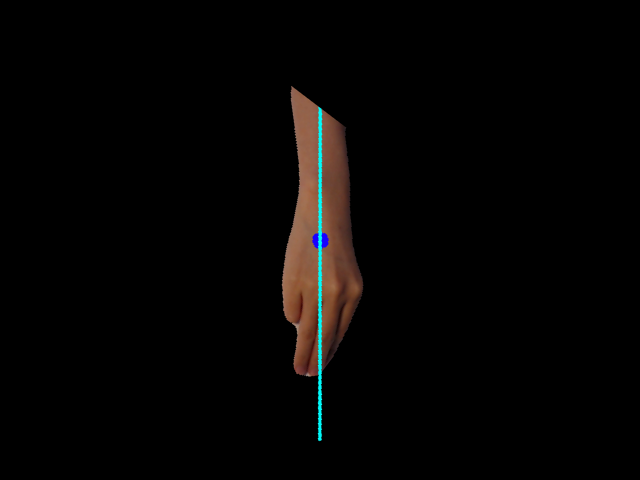
\includegraphics[width=5cm]{fig7/4-a.png} \\
\end{tabular}

 \caption{The results for orientation detection}
 \label{fig:mom2}
\end{figure}

\subsection{Hand detection}
Then we have to extract only hand region. If there are long arms, we may not classify the gesture correctly. We modified the method introduced by \cite{ra11}. The method is first detect the skin region by color (HSV), and then detect the wrist end. Wrist end is detected by the simple method as follows:
Fig.\ref{fig:handim} shows the image of the hand. First, we calculate the pixels on boundaries, up, down, left, right. 
We can assume the most largest among up, down, left and right is the wrist side. This is because the author of \cite{ra11} and we assume hand is inside of the image, but human itself is not. Then, they detect the wrist end using intensity historgam. 
\par
However, the wrist detection does not work well because the paper assumes the hand gesture as spray hand and so the palm is always the widest. 
In our case, palms are not fully opened so it is difficult to detect hand region as it is. 
So we rotate the image along the axis so that we can assume the wrist is always 'up' side and the most left or right part tend to be the palm region.
Fig.\ref{fig:handex}  can detect wrist by our method but not the proposed method. In this case, the proposed method detects the wrist side correctly, but it will calculate slope with either
wrist (blue dot) or fingertip (near yellow dot). Then proposed method does not work.
Our method is as follows.
\begin{enumerate}
  \item Find skin color area
  \item Find orientation of the skin area and rotate
  \item Assume up side is wrist
  \item Find wrist end and crop
\end{enumerate}
Even though we improve the method, in case the skin detection fails and the hand become smaller of the palm is too small to be a widest length, in that case, we simply extract 1/4 of the all of the region.
\subsection{Result}
Fig.\ref{fig:hands} shows the results of the hand detection.
As we can see, the hands are correctly detected.

\begin{landscape}
\begin{figure}[htbp]
 \centering
 \begin{tabular}{ccccccc}
 & 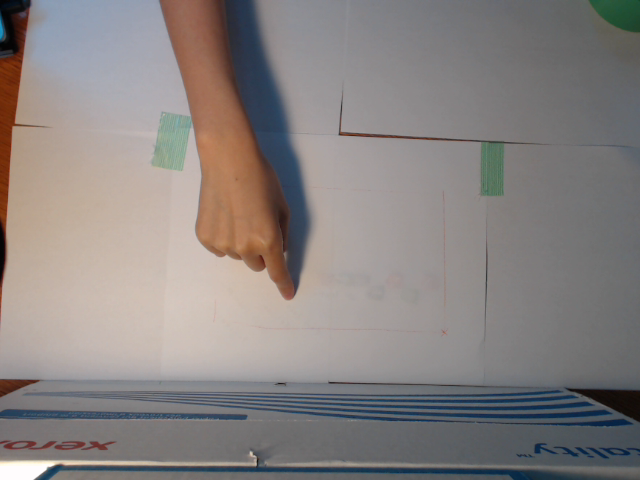
\includegraphics[width=4cm]{fig1/a.png} & $\rightarrow$ &
   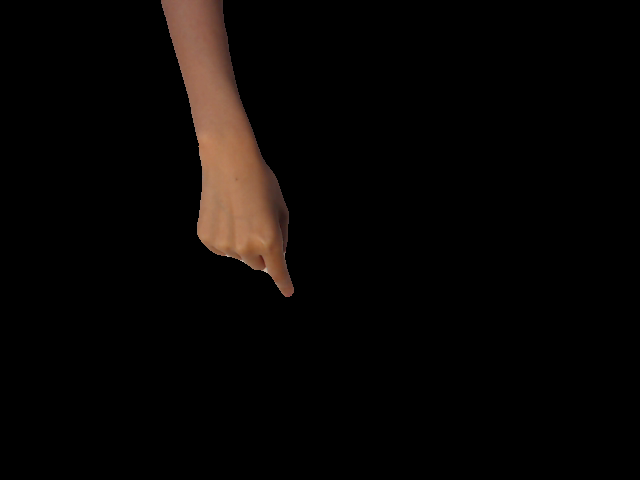
\includegraphics[width=4cm]{fig1/b.png} & $\rightarrow$ &
   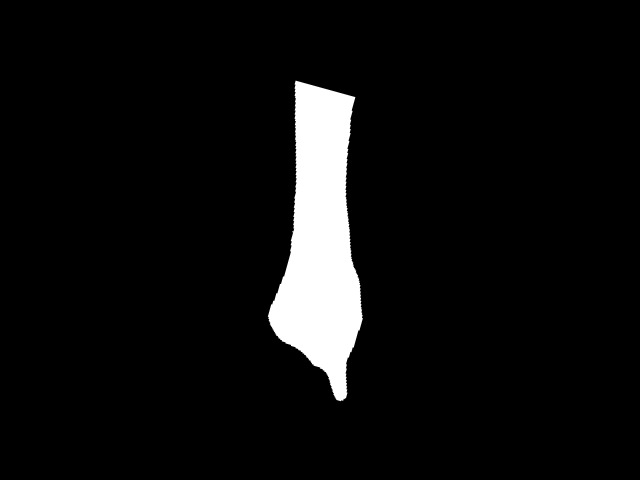
\includegraphics[width=4cm]{fig1/c.png} & $\rightarrow$ \\
& & & Skin color detection & & Major Axis detection \\
 $\rightarrow$ &
   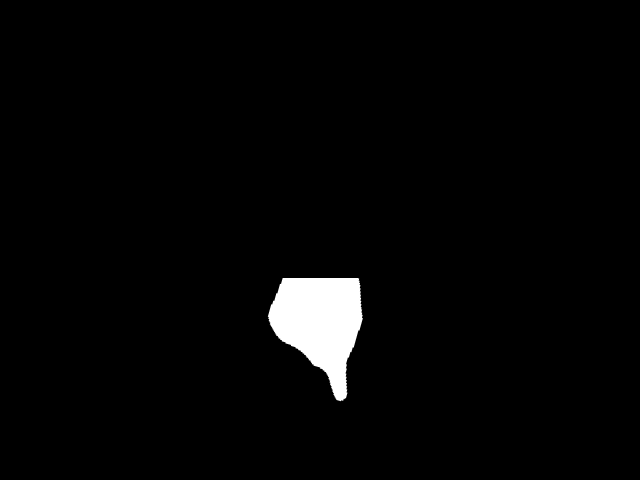
\includegraphics[width=4cm]{fig1/d.png} & $\rightarrow$ &
   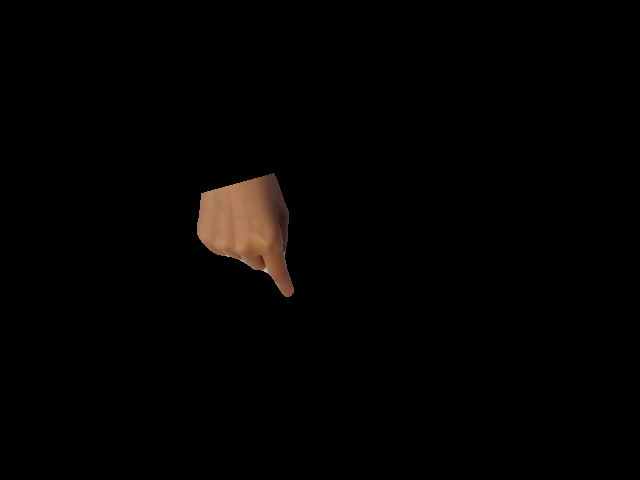
\includegraphics[width=4cm]{fig1/e.png} \\
	 & Wrist detection & & Hand mask
\end{tabular}

 \caption{Overview of hand detection}
 \label{fig:hand}
\end{figure}
\end{landscape}

\begin{landscape}
\begin{figure}[htbp]
 \centering
 \begin{tabular}{lllll}
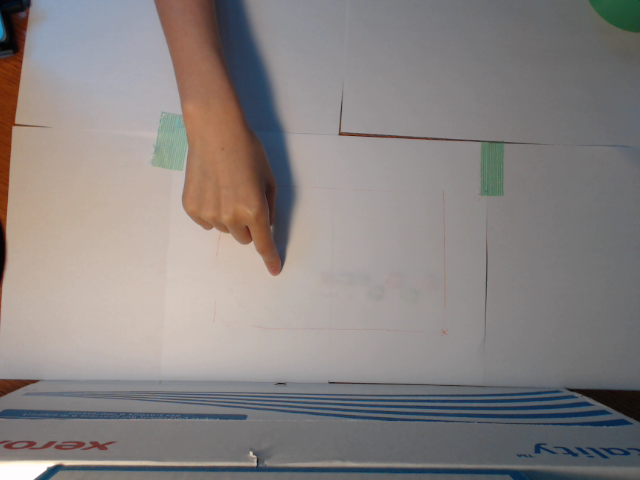
\includegraphics[width=3.5cm]{fig4/1-a.png} &
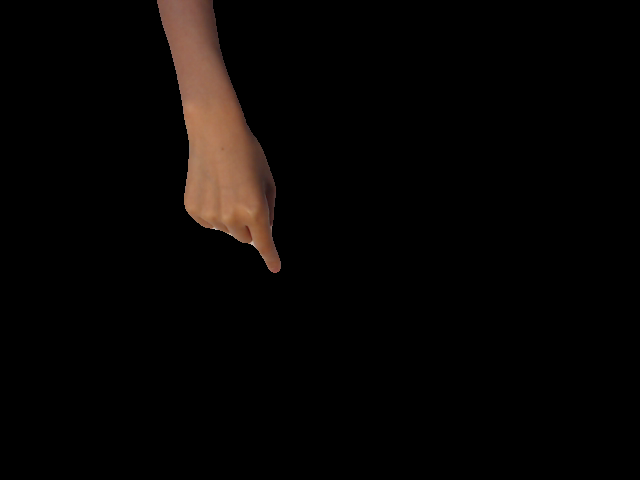
\includegraphics[width=3.5cm]{fig4/1-b.png} &
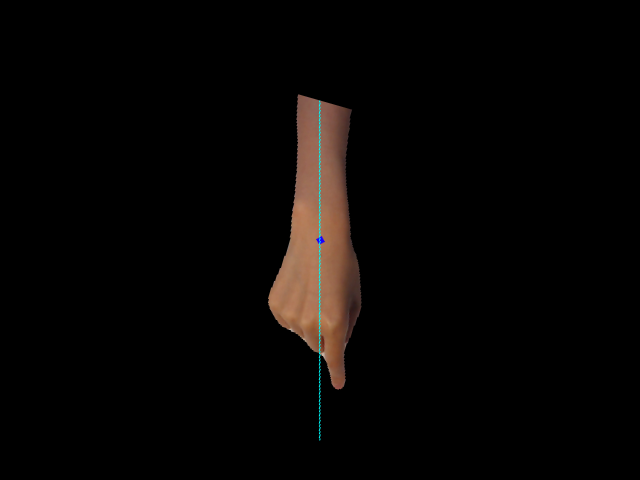
\includegraphics[width=3.5cm]{fig4/1-c.png} &
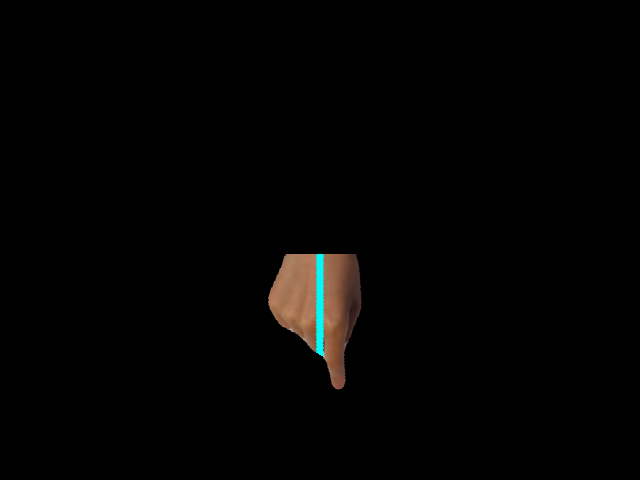
\includegraphics[width=3.5cm]{fig4/1-d.png} &
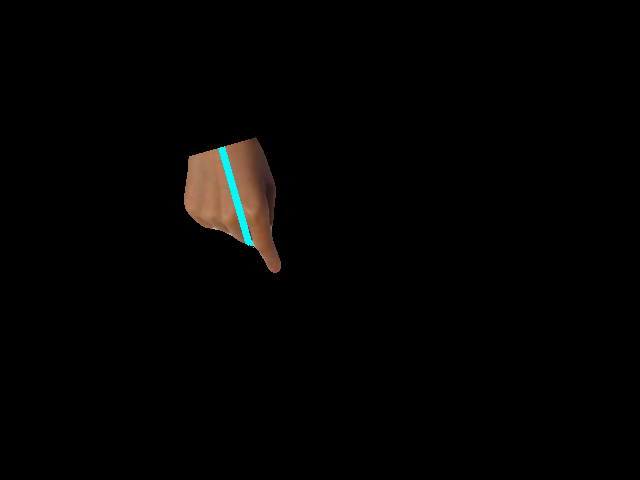
\includegraphics[width=3.5cm]{fig4/1-e.png} \\
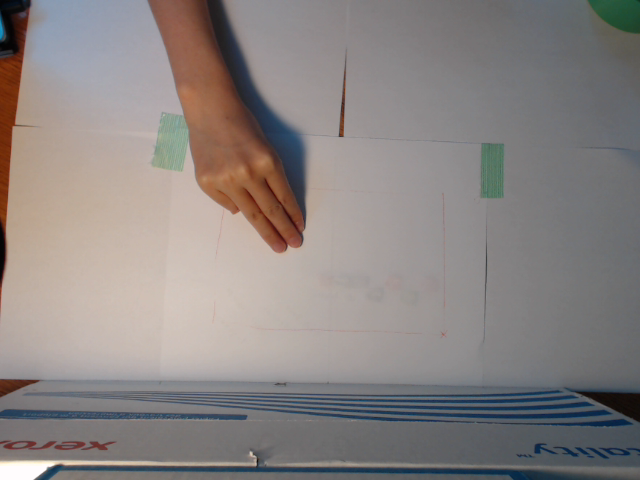
\includegraphics[width=3.5cm]{fig4/2-a.png} &
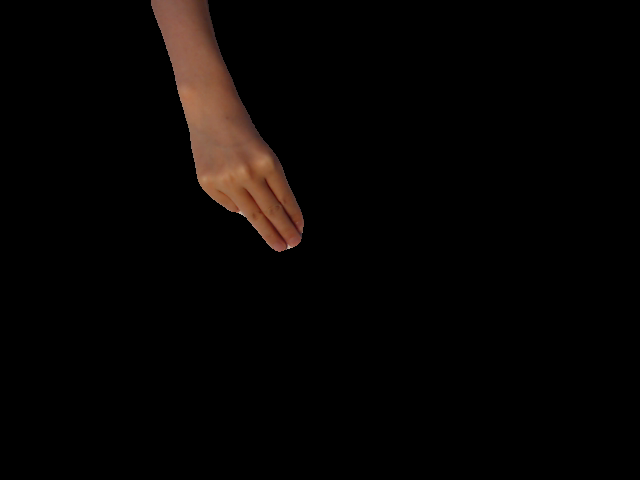
\includegraphics[width=3.5cm]{fig4/2-b.png} &
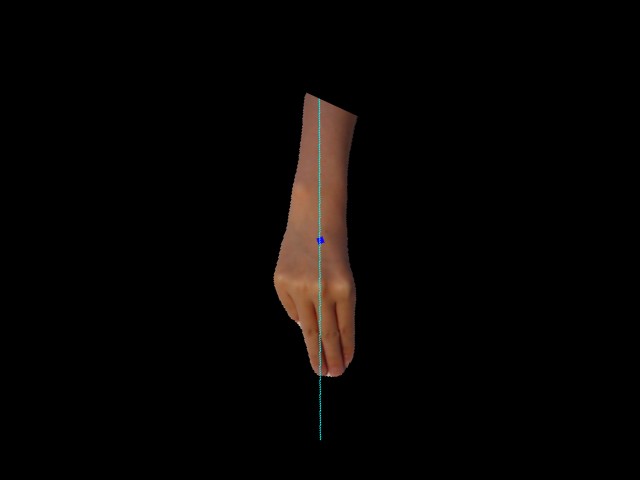
\includegraphics[width=3.5cm]{fig4/2-c.png} &
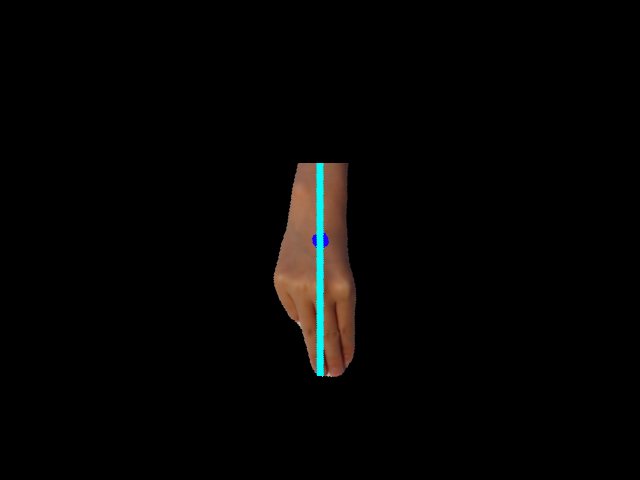
\includegraphics[width=3.5cm]{fig4/2-d.png} &
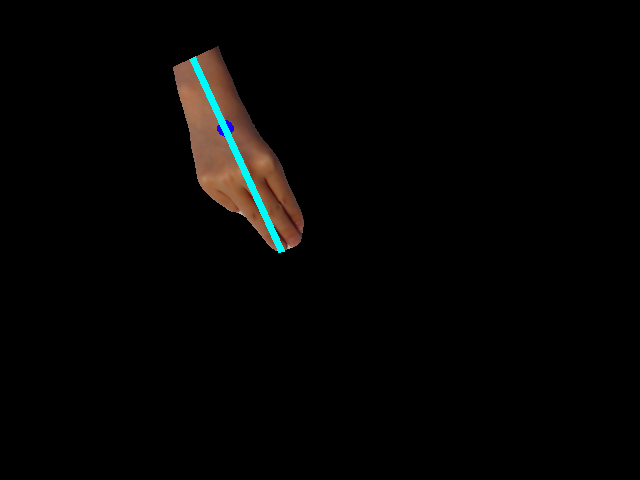
\includegraphics[width=3.5cm]{fig4/2-e.png} \\
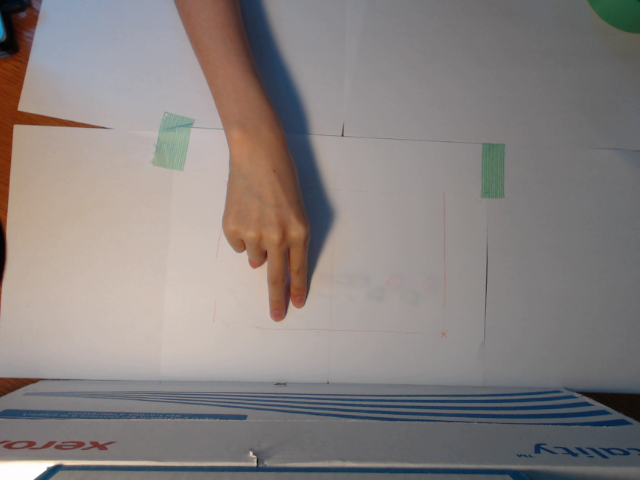
\includegraphics[width=3.5cm]{fig4/3-a.png} &
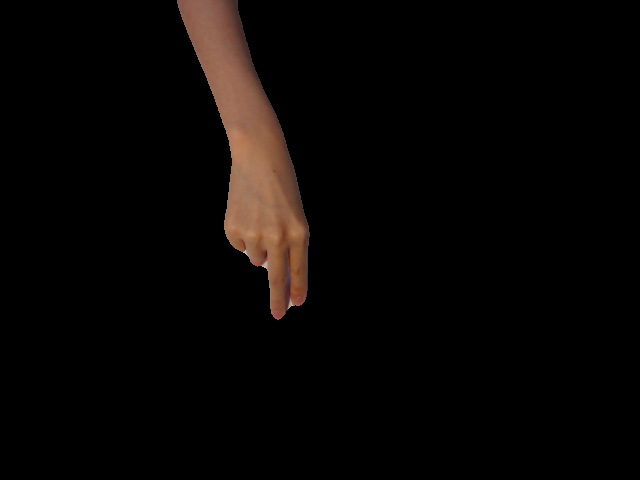
\includegraphics[width=3.5cm]{fig4/3-b.png} &
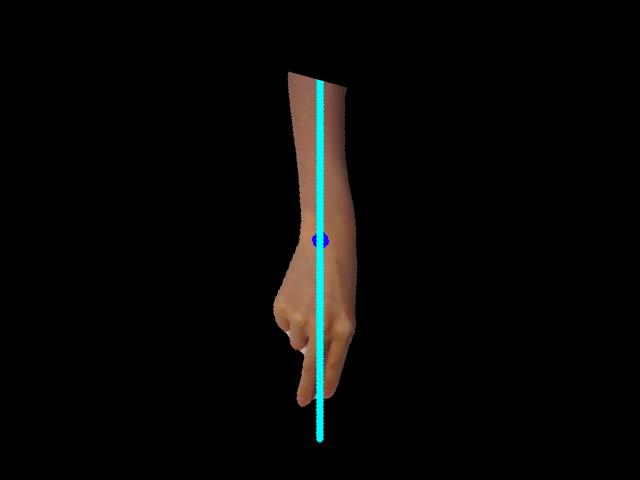
\includegraphics[width=3.5cm]{fig4/3-c.png} &
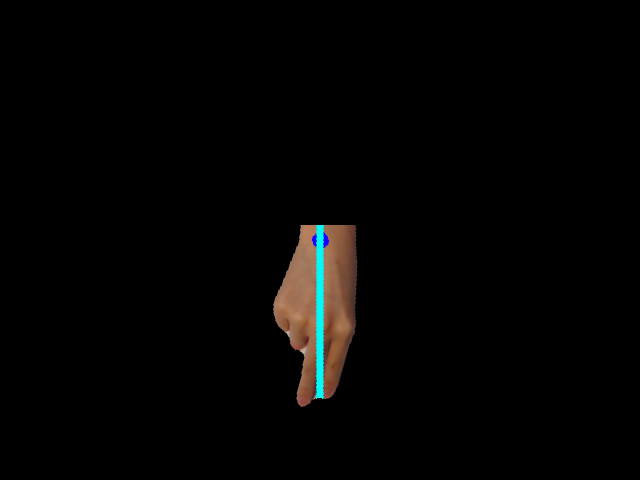
\includegraphics[width=3.5cm]{fig4/3-d.png} &
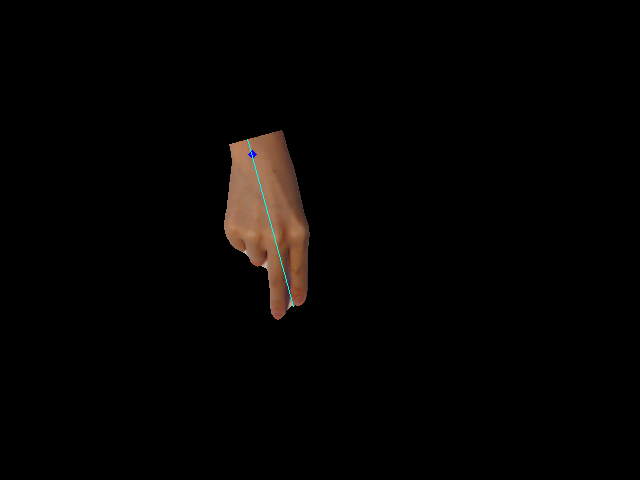
\includegraphics[width=3.5cm]{fig4/3-e.png}
\end{tabular}

 \caption{The results of hand detection}
 \label{fig:hands}
\end{figure}
\end{landscape}
